%%
%% This is file `sample-sigchi.tex',
%% generated with the docstrip utility.
%%
%% The original source files were:
%%
%% samples.dtx  (with options: `sigchi')
%% 
%% IMPORTANT NOTICE:
%% 
%% For the copyright see the source file.
%% 
%% Any modified versions of this file must be renamed
%% with new filenames distinct from sample-sigchi.tex.
%% 
%% For distribution of the original source see the terms
%% for copying and modification in the file samples.dtx.
%% 
%% This generated file may be distributed as long as the
%% original source files, as listed above, are part of the
%% same distribution. (The sources need not necessarily be
%% in the same archive or directory.)
%%
%% The first command in your LaTeX source must be the \documentclass command.
\documentclass[sigconf,review]{acmart}
\usepackage{booktabs}
\usepackage{todonotes}
\usepackage{multirow}
%%
%% \BibTeX command to typeset BibTeX logo in the docs
\AtBeginDocument{%
  \providecommand\BibTeX{{%
    \normalfont B\kern-0.5em{\scshape i\kern-0.25em b}\kern-0.8em\TeX}}}

%% Rights management information.  This information is sent to you
%% when you complete the rights form.  These commands have SAMPLE
%% values in them; it is your responsibility as an author to replace
%% the commands and values with those provided to you when you
%% complete the rights form.
\setcopyright{acmcopyright}
\copyrightyear{2018}
\acmYear{2018}
\acmDOI{10.1145/1122445.1122456}

%% These commands are for a PROCEEDINGS abstract or paper.
\acmConference[Woodstock '18]{Woodstock '18: ACM Symposium on Neural
  Gaze Detection}{June 03--05, 2018}{Woodstock, NY}
\acmBooktitle{Woodstock '18: ACM Symposium on Neural Gaze Detection,
  June 03--05, 2018, Woodstock, NY}
\acmPrice{15.00}
\acmISBN{978-1-4503-XXXX-X/18/06}


%%
%% Submission ID.
%% Use this when submitting an article to a sponsored event. You'll
%% receive a unique submission ID from the organizers
%% of the event, and this ID should be used as the parameter to this command.
%%\acmSubmissionID{123-A56-BU3}

%%
%% The majority of ACM publications use numbered citations and
%% references.  The command \citestyle{authoryear} switches to the
%% "author year" style.
%%
%% If you are preparing content for an event
%% sponsored by ACM SIGGRAPH, you must use the "author year" style of
%% citations and references.
%% Uncommenting
%% the next command will enable that style.
%%\citestyle{acmauthoryear}

\newcommand{\theArticle}{\textit{Towards innovation measurement in the software industry}}
%%
%% end of the preamble, start of the body of the document source.
\begin{document}

%%
%% The "title" command has an optional parameter,
%% allowing the author to define a "short title" to be used in page headers.
\title{The Impact of a Proposal for Innovation Measurement in the Software Industry}

%%
%% The "author" command and its associated commands are used to define
%% the authors and their affiliations.
%% Of note is the shared affiliation of the first two authors, and the
%% "authornote" and "authornotemark" commands
%% used to denote shared contribution to the research.

%\author{Nauman bin Ali}
%\orcid{0000-0001-7266-5632}
%\affiliation{%
%  \institution{Blekinge Institute of Technology}
%  \country{Sweden}}
%\email{nauman.ali@bth.se}

%\author{Henry Edison}
%\affiliation{%
%  \institution{Lero, NUI Galway}
%  \country{Ireland}}
%\email{henry.edison@nuigalway.ie}

%\author{Richard Torkar}
% \orcid{0000-0002-0118-8143}
% \affiliation{
% \institution{Chalmers and University of Gothenburg}
% \country{Sweden}
% }
% \affiliation{
% \institution{Stellenbosch Institute for Advanced Study (STIAS)}
% \country{South Africa}
% }
% \email{torkarr@chalmers.se}

\author{First Author}
\email{first.author@company.com}
\affiliation{%
  \institution{Company Name}
  \streetaddress{Street Address}
  \city{City}
    \postcode{Code}
   \country{Country}}


\author{Second Author}
\email{second.author@article}
\affiliation{%
  \institution{University Name}
  \streetaddress{Street}
  \city{City}
    \postcode{37 179}
   \country{Country}}
   
\author{Third Author}
\email{third.author@article}
\affiliation{%
  \institution{University Name}
  \streetaddress{Street}
  \city{City}
    \postcode{37 179}
   \country{Country}}


%%
%% By default, the full list of authors will be used in the page
%% headers. Often, this list is too long, and will overlap
%% other information printed in the page headers. This command allows
%% the author to define a more concise list
%% of authors' names for this purpose.
\renewcommand{\shortauthors}{Ali et al.}

%%
%% The abstract is a short summary of the work to be presented in the
%% article.



\begin{abstract}
\textbf{Background:} Measuring an organization's capability to innovate and assessing its innovation output and performance is a challenging task. Previously, a comprehensive model and a suite of measurements to support this task were proposed. The contribution was based on surveys of relevant literature (using a systematic literature review) and practitioners' opinion (elicited using questionnaire and interviews).
\textbf{Aims:} In the current paper, seven years since the publication of the paper titled \theArticle, we have reflected on the impact of the work.
\textbf{Method:} We have mainly relied on quantitative and qualitative analysis of the citations of the paper using an established classification schema.
\textbf{Results:} We found that the article has had a significant scientific impact (indicated by the number of citations), i.e., (1) cited in literature from both software engineering and other fields, (2) cited in grey literature and peer-reviewed literature, and (3) substantial citations in literature not published in the English language. However, we consider a majority of the citations in the peer-reviewed literature (75 out of 116) as neutral, i.e., they have not used the innovation measurement paper in any substantial way. All in all, 38 out of 116 have used, modified or based their work on the definitions, measurements or the model proposed in the paper. This analysis revealed a significant weakness of the citing work, i.e., among the citing papers, we found only two explicit comparisons to the innovation measurement proposal, and we found no papers that identify weaknesses of said proposal. 
\textbf{Conclusions:} This work highlights the continued need for improving the practical impact of our research, being cautious of relying on solely the number of citations for impact, and the need for further improving and supporting the peer-review process to identify unwarranted citations in papers.

\end{abstract}

%%
%% The code below is generated by the tool at http://dl.acm.org/ccs.cfm.
%% Please copy and paste the code instead of the example below.
%%

\begin{CCSXML}
<ccs2012>
<concept>
<concept_id>10011007.10011074</concept_id>
<concept_desc>Software and its engineering~Software creation and management</concept_desc>
<concept_significance>500</concept_significance>
</concept>
</ccs2012>
\end{CCSXML}

\ccsdesc[500]{Software and its engineering~Software creation and management}

%%
%% Keywords. The author(s) should pick words that accurately describe
%% the work being presented. Separate the keywords with commas.
\keywords{innovation, impact, relevance, measurement}


%%
%% This command processes the author and affiliation and title
%% information and builds the first part of the formatted document.
\maketitle


\section{Introduction}\label{sec:intro}
In the past, companies had relied mainly on cost and lead time reduction and quality improvement to strengthen their competitiveness. While quality is a necessity, today it is not sufficient. Companies must continuously innovate; develop new processes, and deliver new products to achieve and sustain a competitive advantage. Otherwise, they tend to lose their position to new and emerging startups that have innovative offerings. Such turnover signifies the importance of sustained innovation instead of happen-stance innovation. For sustained innovation to become a reality, a better understanding of innovation is required, which, we would argue, is possible only when innovation is measured.

The importance of innovation measurement is also well recognised in industry. The Boston Consulting Group's survey~\cite{andrew08} revealed that most executives believe that their companies should measure innovation as rigorously as core business operation, but less than half of companies actually do so. There is little consensus on how innovation measurement should be carried out. Each definition of innovation signifies a different aspect of innovation, e.g., considering only a selection of perspectives, levels, and types. This, in turn, determines what is considered elements of innovation and how these are measured.

Organisations require means not only to measure their innovative output but also to assess their ability and capacity to innovate. Measurement helps to understand better and evaluate the consequences of the initiatives geared towards innovation. Furthermore, like any other measurements, these will allow organisations to specify realistic targets of innovation and to identify and resolve problems hindering progress towards goals, making decisions, and continuously improving the ability to innovate.

Given the importance of innovation measurement for the software industry and the lack of a systematic approach for it, a conceptual model of the key measurable elements of innovation was proposed. Furthermore, a suite of metrics for the evaluation of innovation determinants, inputs, outputs, and performance was aggregated and categorised. The contribution was reported in an article published in the \textit{Journal of Systems and Software} in the year 2013~\cite{EdisonAT13}.

The paper has collected a relatively high number of citations, which makes it an interesting candidate for a reflections paper in ESEM. Also the methods used in \theArticle{} (a combination of systematic literature review and survey research) makes the paper relevant for a reflection paper at ESEM. In this regard, we raise and answer the following questions in this study:

What is the impact of \theArticle? 
\begin{enumerate}
    \item Who cites the paper? We analyse the metadata of citing papers to characterise them, in terms of discipline (software engineering or others), type of publications (peer-reviewed and non-peer-reviewed) and venues of publications.
    \item Why is the paper cited? We analyse the full-text of peer-reviewed publications to understand how the citing papers have used the innovation measurement proposal. We also attempt to identify evidence of any industrial application of that work.
\end{enumerate}

The remainder of the paper is structured as follows: Section~\ref{sec:sumpaper} summarizes the contribution of \theArticle. Section~\ref{sec:method} describes our approach to understand the impact of \theArticle. In Section~\ref{sec:whocites}, we present an overview of the citations to \theArticle. Section~\ref{sec:soa} discusses the research identified in Section \ref{sec:whocites} that has extended the innovation measurement proposal. In Section~\ref{sec:impact}, we discuss the research which documents the use of our work in industrial settings. Section~\ref{sec:fw} concludes the paper with some suggested directions for future research.

\section{A summary and main contributions of \theArticle} %\todo{Henry}
\label{sec:sumpaper}
In \theArticle, the aim was to establish the state of the art of innovation measurement and to capture the state of the practice of innovation measurement in the software industry. A systematic literature review (SLR)~\cite{kitchenham07} was conducted to establish the state of the art of innovation measurement, followed by a web-based questionnaire~\cite{kasunic05} and face-to-face interviews~\cite{creswell09} to collect the opinions of software industry practitioners and academics. In total, 13,401 articles from seven digital libraries (Compendex, Scopus, IEEEXplore, ACM Digital Library, ScienceDirect and Business Source Premier) were retrieved. After applying inclusion\slash exclusion criteria, 204 papers were accepted as primary studies. 94 completed the questionnaire out of the total of 145 who responded, thus the completion rate was 64\%. Additionally, four industry practitioners (middle managers) and three academics with a close relationship with industry were interviewed in this study. 

The review showed that there were 41 definitions of innovation found in the literature which highlight 4 important attributes to measure: 
\begin{itemize}
    \item Impact of innovation on the market and technology, e.g., incremental or radical innovation, market or technological breakthrough.
    \item Types of innovation, e.g., product (new or significantly improved products), process (new or significantly improved design, analysis, or development method), market (new or significantly improved marketing methods, strategies, and concept in product design or packaging, placement, promotion, or pricing), and organisation innovation (new or significantly improved organisation methods, e.g., business practices, workplace organisation or external relations.
    \item Degree of novelty, e.g., new to the firm, new to the market, new to the world, and new to the industry.
    \item Nature of process: iterative process.
\end{itemize}

While 28 determinants of innovation had been reported in literature, only 7 of them were studied in the software industry: internal collaboration, customer orientation, champions, human resources, strategy, networking, and leadership. In total, 232 metrics had been proposed to measure innovation at a firm (88\%), industry (1\%), or regional level (11\%). However, only 37\% of them have been statistically validated, and 58\% had never been used in practice. The review also identified 13 innovation measurement frameworks. Most of these frameworks focused on technological breakthrough (eight frameworks). Out of these frameworks, only one framework had been studied at software companies. 

The results of the interview and the questionnaire were consistent with the view of the impact, types, and the dimension of the novelty of innovation. The experts and respondents with management and executive roles perceived innovation at a much broader level and emphasised the market and organisation innovations by using abstract concepts like value creation and need fulfilment. They looked at the purpose and goal to define what may be considered as innovation. The respondents with technical roles had a strong inclination on product innovation as they were mainly involved in product development.

The questionnaire and interview results showed an agreement regarding the importance of innovation measurement, but the practice was found lagging. A majority of respondents and experts reported a lack of an explicit innovation strategy and measurement program in their companies. Moreover, in terms of innovation measurement the following challenges were identified:

\begin{itemize}
    \item Lack of consistent definition of innovation. Definitions are fundamental as they affect the measurement program and help provide a common understanding.
    \item Lack of meaningful metrics. For example, R\&D measures (e.g., the percentage of sales spent on R\&D, number of R\&D staff) only focus on input and may not be applicable in small and medium enterprises. Similarly, the IPR-based measures (e.g., patent counts, and citation-based data, etc.) may no represent innovation at all, rather it could be used as a way to prevent a competitor from exploiting opportunities.
    \item Lack of frameworks to guide innovation measurement. Measurement frameworks consist of a set of related metrics, data collection mechanism, and data use inside a company. However, as there is no clear understanding of what innovation is, there is also no agreement on what metrics should be collected.
\end{itemize}

Using the different perspectives of innovation and the key aspects of innovation measurement as identified by the systematic literature review, an innovation measurement model, as shown in Figure~\ref{fig:im_model}, was developed. This model was further refined after preliminary evaluation by academics and practitioners. From the outset, the model identifies three main elements of measurement: innovation capability, innovation output, and impact of innovation. Unlike the current strict reliance on sales as the sole measure for innovation, which may produce negative effects on the innovation climate of the organisation, this model highlights the opportunity for a more comprehensive approach towards innovation measurement. Each of these aspects identified in the model can be measured quantitatively (using both objective and subjective metrics). Metrics for each of these aspects identified from literature were aggregated and categorised.

\begin{figure}
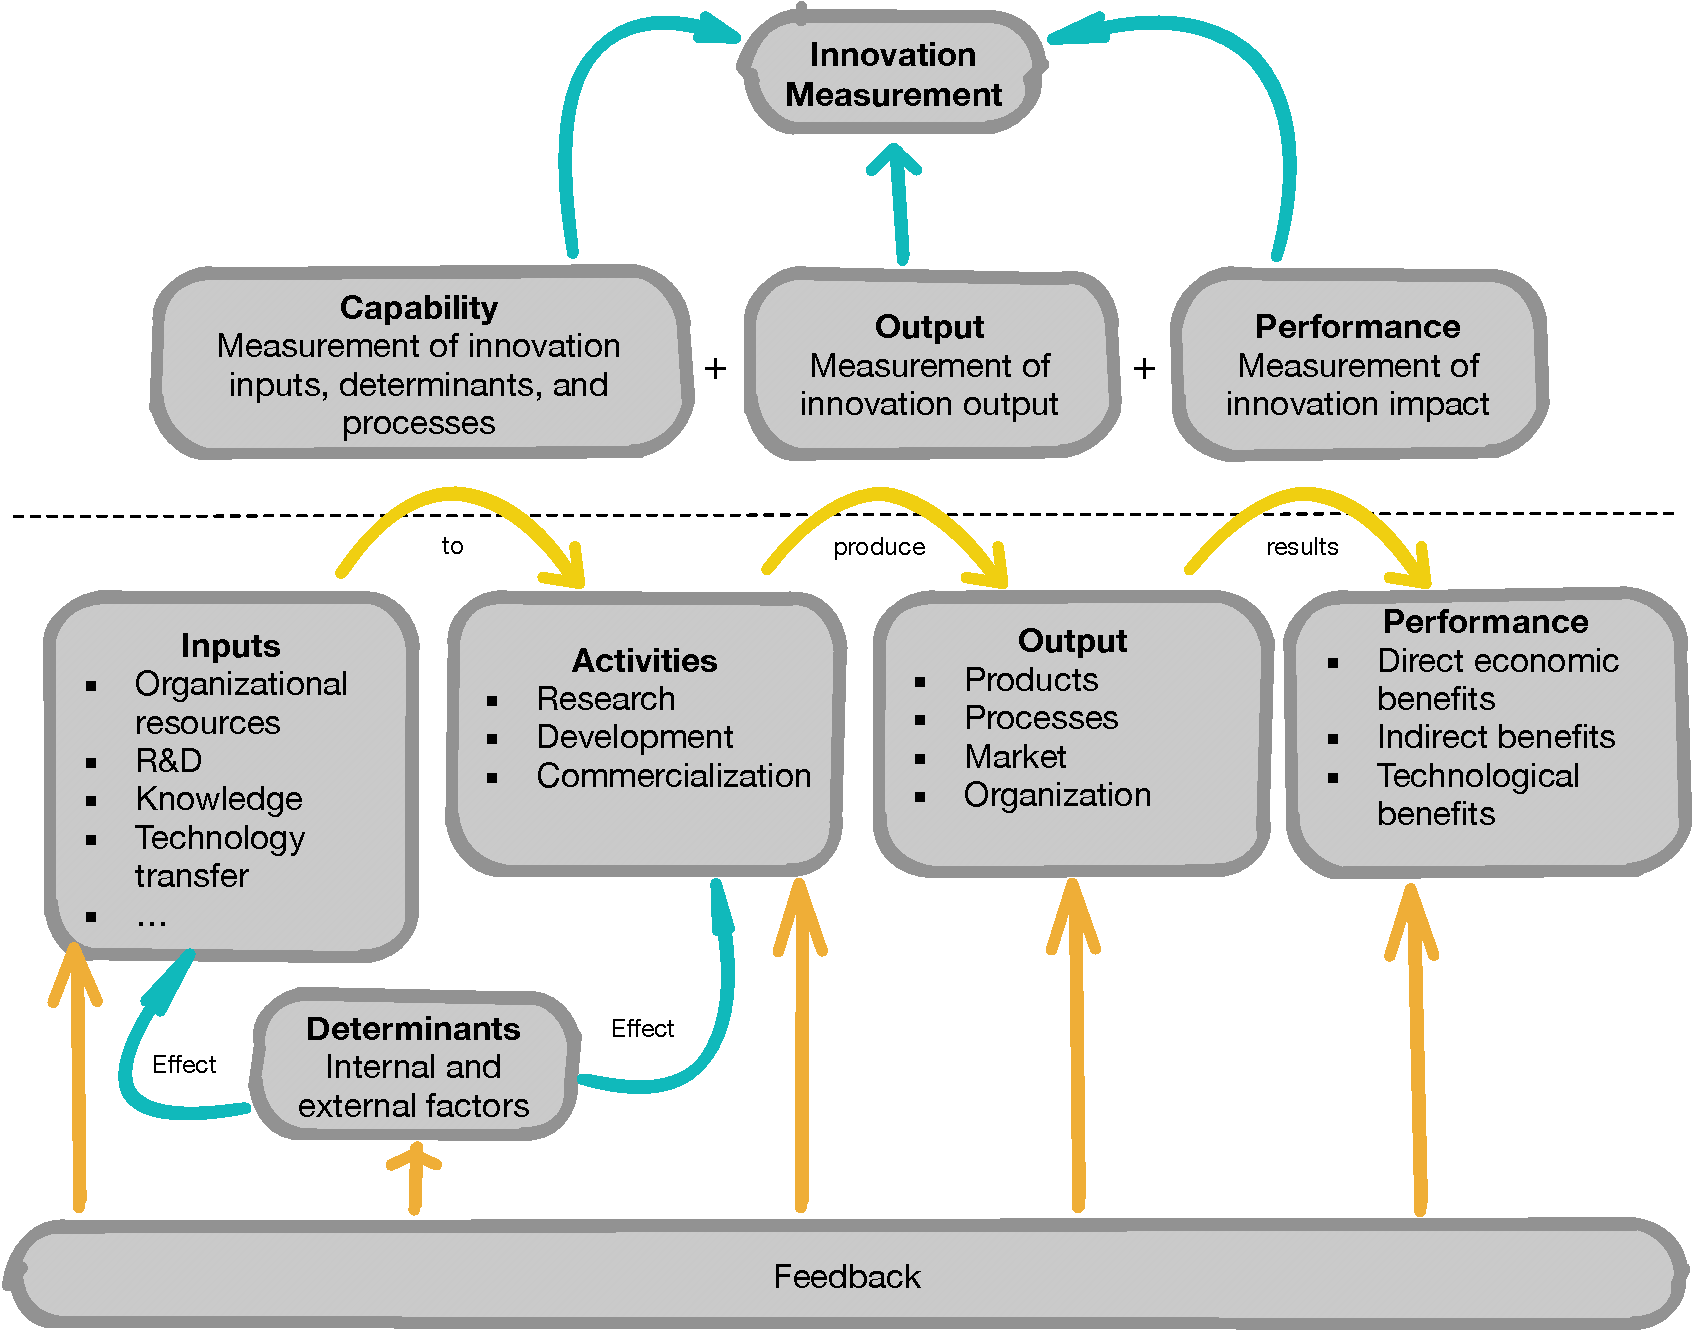
\includegraphics[width=\columnwidth]{Figures/IM.pdf}
\caption{Innovation Measurement Model as presented in the paper \theArticle.}
\label{fig:im_model}
\end{figure}

In terms of implications, the paper made three contributions to both research and practice. First, this study aggregated the available empirical evidence reported in the literature to establish state of the art in innovation measurement through an extensive literature review. The outcome of this review contributed to the existing body of knowledge in the form of an innovation measurement model, enumeration of metrics and their classification based on what aspect of innovation they are used to measure. The second contribution was to provide an innovation measurement model, which was founded in empirical research and had been evaluated by experts. The model captures several dimension of innovation. Industry practitioners could use these findings to reflect on their experience on innovation measurement to minimise the challenges in their contexts. Finally, the study provided future direction for innovation measurement research.


\section{Methodology}\label{sec:method} %\todo{Nauman}
For understanding the impact of \theArticle, we have relied on the classification schema for academic citations proposed by \citet{teufel2006annotation}. We also considered the taxonomy proposed by \citet{bornmann2008citation}. However, based on a pilot application, we found \citet{teufel2006annotation} more straight forward and sufficient for our analysis. The decision is further supported by prior experience of using Bornmann and Daniel's taxonomy in software engineering literature~\cite{poulding2015using}.

The categories in the schema we used are listed and briefly described in Table~\ref{tab:CitationCategories}. To separate any industrial application of the work we added a separate category. 

On February 24, 2020, the \theArticle{} had over 72 citations in Science Direct and Scopus, 61 in Web of Science Core Collection, and 234 in Google Scholar. To get a relatively complete picture of how this work has impacted further research, we decided to analyse the 234 citations on Google Scholar. 

In a pilot, the first two authors classified ten randomly selected articles and discussed the use of categories. Thereafter, they divided the 234 articles among them and  independently classified them. The procedure followed is briefly summarized below: 
\begin{itemize}
\item Exclude citations where the full-text is not available. 
\item Exclude articles which are not written in English.
\item Exclude articles  that do not cite \theArticle{} in the full-text.
\item From the title, abstract and the publication venue judge the discipline of the publication (e.g. software industry, manufacturing, farming or automotive).
\item Only for conference papers and journal article, search for the citation to \theArticle{} in the full text, for each citation in the paper  read the entire paragraph containing it to understand the context, then classify the citation based on categories in Table~\ref{tab:CitationCategories}.
\end{itemize}
 


\begin{table*}
	\caption{Categories of citing papers from \citet{teufel2006annotation}}\label{tab:CitationCategories}
	\begin{tabular}{llp{12cm}}
		\toprule
		\textbf{Category}            & \textbf{Sub-category }& \textbf{Description}                                                                                                            \\ \midrule
		Weakness            & Weak         & Weakness of the approach pursued in \theArticle, Weakness in the definition, model, entities, attributes, or measurements of innovation as proposed in \theArticle                                                                                              \\
		\midrule
		Contrast/Comparison & CoCoGM       & Contrast\slash Comparison in Goals or Methods (neutral)                                                                    \\
		& CoCoR0       & Contrast\slash Comparison in Results (neutral)                                                                               \\
		& CoCo-        & Unfavourable Contrast\slash Comparison (current work is better than the work in \theArticle)                                            \\
		& CoCoXY       & Contrast between a cited method and the method in \theArticle                                                                                     \\
		
		\midrule
		Positive sentiment  & PBas         & author uses the work in \theArticle{} as a starting point                                                                               \\
		& PUse         & author uses definitions\slash models\slash measures                                                                                      \\
		& PIUse\footnote{We have added this category}         & author uses the work in \theArticle{} in industrial settings \\
		& PModi        & author adapts or modifies definition\slash model\slash measurements presented in \theArticle                                                                            \\
		& PMot         & this citation is positive about approach or problem addressed in \theArticle{} (used to motivate work in current paper)                 \\
		& PSim         & author's work and the work in \theArticle{} are similar                                                                               \\
		& PSup         & author's work and the work in \theArticle{} are compatible\slash provide support for each other                                           \\
		
		\midrule
		Neutral             & Neut         & Neutral description of cited work, or not enough textual evidence for above categories.\\
		\bottomrule
	\end{tabular}
\end{table*}

\section{Overview of the papers citing \theArticle}\label{sec:whocites} %\todo{Nauman} %covers: Who found it relevant (would be good to have some qualitative data on how they ref the paper). Why did so many cite it?}

The 234 citations to \theArticle{} were analysed using the process described in Section~\ref{sec:method}. Figure~\ref{fig:selection} provides the results of the selection steps. In total 118 citations were excluded from further analysis. We considered 54 as grey literature, i.e., books, technical reports, and theses. A majority, i.e., 42 of the 54 citations classified as grey literature, were masters or doctoral theses. Similarly the remaining 64 of the 118 citations were excluded for other reasons (language of the publication, inaccessible full-text, incorrect citation, or duplicate citations). A clear majority 52 of the 64 citations excluded in this group were not read in full-text as they were not written in English.

Two interesting results emerge from this data: (1) a significant number of publications not written in English have cited \theArticle, and (2) almost an equal number of citations are from grey literature. This indicates that systematic literature reviews in software engineering, like in medicine, should also develop a strategy to consider such literature, or at the very least consider the impact of not including such literature in SLRs.

\begin{figure}
	\begin{center}
		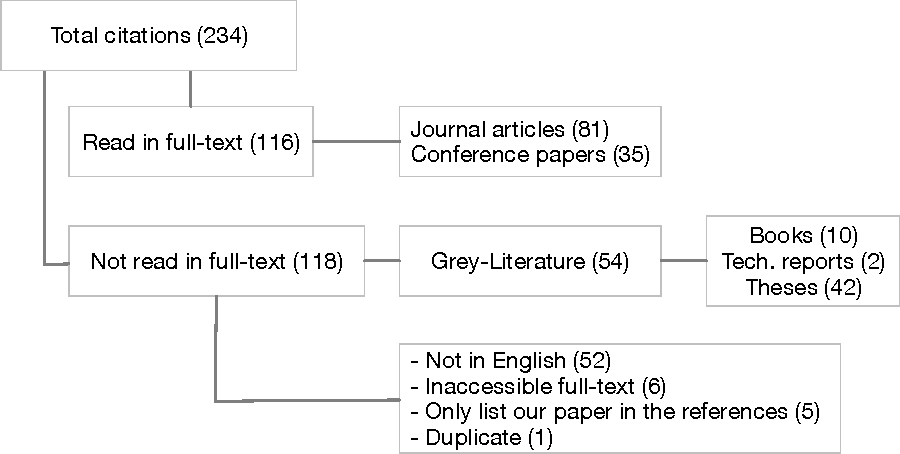
\includegraphics[width=0.38\textwidth,height=\textheight,keepaspectratio]{Figures/Citations.pdf}
	\end{center}
	\caption{Results of applying the selection criteria on the citations}
	\label{fig:selection}
\end{figure}

The remaining 116 of the 234 citing papers were read in full-text. Of these 81 were journal articles and 35 were conference papers citing \theArticle. This is an interesting result in itself as \theArticle{} is getting significantly more citations from journal articles and grey literature than conference papers. When looking at the publication forums from software engineering and other fields we see a different pattern. In SE, 24 of the 44 (55\%) citing papers are journal articles and remaining 20 (45\%) are conference papers. Where as in the 72 citing articles from other fields 57 (80\%) are journal articles and 15 (20\%) are conference papers. We speculate that this may be an artifact of different traditions of publications in different fields i.e. other fields may not have similar tradition of conference proceedings or even a similar frequency of conferences.

The analysis of the use of \theArticle{} in 116 conference papers and journal articles is summarized in Table \ref{tab:CitationAnalysis}. Only eight self citations were identified. 

\theArticle, proposed a model and metrics based on a consolidation of research from other fields for software development field. However, it is interesting to observe that the article has been cited frequently in literature from outside software engineering. Only 44 of the 116 (38\%) of the publications are on topics related to software development. A majority, 67 of the 116 (62\%) of the citing articles have no stated connection to the context of the software industry. These articles encompass several diverse fields including the following: automotive, banking, economics, farming, forestry, health sector, human resources, logistics, manufacturing, mechatronics, NGOs, oil industry, politics, restaurants, and transportation.  A more detailed analysis of the reasons for the citations will help in understanding the reason for this disparity.

Overall, in terms of the categories of the citing article (please see Table~\ref{tab:CitationCategories} for a listing and the definitions of the categories) 75 of 116 (65\%) are neutral, 38 of 116 (32\%) are neutral, and only 2 out of 116 (i.e., less than 1\%), present a comparison\slash contrast. Surprisingly, we did not find any papers identifying or discussing a weakness of the research documented in \theArticle.
 
We expected that the number of citing articles in different categories will be different for literature from software engineering research and other fields. However, similar patterns of citation appear both in and outside software engineering. In software engineering literature, of the 44 citing papers, 17 (39\%) were positive, 27 (61\%) were neutral, while no comparison\slash contrast or weaknesses of \theArticle{} could be found. Among the 72 citing papers from other fields, 21 (29\%) were positive, 48 (67\%) were neutral, while 2 citing papers presented a comparison\slash contrast and no citing papers present any weaknesses of \theArticle. Hence, no discernible difference in citing patterns can be observed. 

A majority, i.e., 21 of the 38 (55\%), citing articles within the `positive' category, used the definition, metrics, or the model as proposed in \theArticle. The next most frequent (12 of the 38 cases in the category, i.e., 32\%) positive use of \theArticle{} was as a starting point or motivation for their work. A few articles also described that they adapted the definitions presented in \theArticle{}, or considered their work similar or supporting the work presented in \theArticle. 

However, we found no documented evidence, in the citing papers, of applying the model or metrics given in \theArticle{} in industry. Perhaps the grey literature, not considered for the detailed analysis in this study, may have reported such a case as an experience report or technical report.

\begin{table*}
	\caption{Results of an analysis of the citing papers}
	\label{tab:CitationAnalysis}
	\begin{tabular}{p{2.5cm}llp{1.5cm}llll}
			\toprule
		& Total & Weak & Comparison / Contrast & Positive                                            & Neutral & Jrnl. & Conf. \\
		\midrule
		&       &      &                       &                                                     &         &         &            \\
		Self citations               & 8     & 0    & 0                     & 2 (PBas:1, PMot:1, PModi:1)                         & 6       & 5       & 1          \\
		From software related fields & 44    & 0    & 0                     & 17 (PBas:4, PModi:2,PUse:7,PMoti:4, PSup:1)         & 27      & 24      & 20         \\
		Others                       & 72    & 0    & 2                     & 21 (PBas:2, PModi:2,PUse:14,PMoti:2,PSim:1, PSup:2) & 48      & 57      & 15         \\
		Total                        & 116   & 0    & 2                     & 38 (PBas:6, PModi:2,PUse:21,PMoti:6,PSim:1, PSup:3) & 75      & 81      & 35        \\ \bottomrule
	\end{tabular}
\end{table*}

\section{Positioning in consideration of the recent state of the art and practice}\label{sec:soa} %\todo{Henry} \todo[inline]{Nauman: I would suggest that there are 44 peer-reviewed articles that cite our paper which we have considered from SE literature. In this section, we can present a brief mapping of these papers e.g. topics of these papers (like open innovation, ecosystems, Lean and agile, startups), research type (empirical, theoretical, ...) etc. In a way covering what has been done in papers that cite our work (thus going in a bit more detail of the 44 papers identified in the previous section). %Open innovation seems to be the area in SE that has been a follow-up of our work.}
Our reading from the 44 citing papers indicate various research areas within SE context, e.g., software measurement, requirement engineering, software ecosystem, and agile development. Open innovation seems to gain more interest from scholars (six papers). %Open innovation is based on outside-in and inside-out knowledge flows that leverages both product and process innovation. 
Innovation stimulus, innovation measurement, and corporate innovation, are the second most reported topics (four papers each). Innovation stimulus focuses on the key factors or determinant of innovation, while the papers in the category ``corporate innovation'' deal with leveraging innovation in large companies. In addition, three papers focused on developing an innovation process model.

In terms of research type, 13 citing studies were theoretical papers (including literature review papers), while 28 were classified as empirical research. All of the empirical research employed qualitative method. Case study was the predominant research method (21 studies), followed by grounded theory (2 studies), survey (2 studies), and then design science, experiment, and interview (with 1 study each). The summary of citing papers in SE and research methods employed is shown in Table~\ref{tab:papers_method}.

\begin{table*}
\caption{Citing papers and research methods employed.}
\label{tab:papers_method}
\begin{tabular}{p{4cm}p{1.7cm}p{1.7cm}p{3cm}lp{1.7cm}}	\toprule
	Theme & \multicolumn{5}{c}{Type of Studies} \\ \cline{2-6}
          & \multirow{2}{*}{\parbox{2.5cm}{Theoretical}} & \multicolumn{4}{c}{Empirical} \\ \cline{3-6}
                         &             & Case Study & Grounded Theory & Survey & Others \\ \midrule
Open Innovation          & 4           & 1          &                 & 1      &                                                           \\
Innovation Stimulus      & 1           & 2          &                 &        & 1                                                         \\
Corporate Innovation     & 1           & 3          &                 &        &                                                           \\
Innovation Measurement   &             & 4          &                 &        &                                                           \\
Innovation Process Model &             & 2          & 1               &        &                                                           \\
Others                   & 7           & 9          & 1               & 1      & 2              
\\ \bottomrule                                          
\end{tabular}
\end{table*}

\section{Expected impact}\label{sec:impact}%\todo{Nauman}
%Here it would be nice to show cases in industry not counting Ericsson. Perhaps we can get it from Section~\ref{sec:whocites}?

Figure~\ref{fig:citationTrend} shows the trend of citations to \theArticle{} as indexed on Google Scholar. According to PlumX Metrics\footnote{Please see the following URL for latest statistics for \theArticle{} \url{https://plu.mx/plum/a/?doi=10.1016/j.jss.2013.01.013&theme=plum-sciencedirect-theme&hideUsage=true}}, in terms of the number of citations provided by Scopus, \theArticle{} is getting more citations than 97\% of the articles published in 2013 in the \textit{Journal of Systems and Software}. The article had an advantage since it was available online already in February 2013. However, \theArticle{} is also doing better than 95\% of the articles published in the \textit{Journal of Systems and Software} in the years 2011--2013.

\begin{figure}
	\begin{center}
		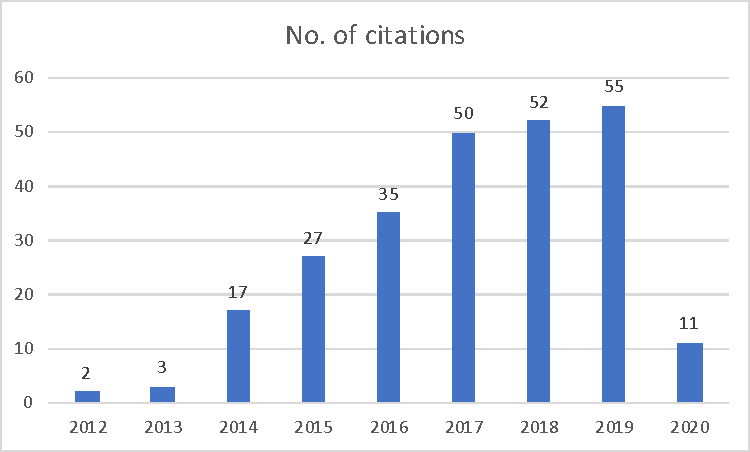
\includegraphics[width=0.45\textwidth,height=\textheight,keepaspectratio]{Figures/CitationsTrend.pdf}
	\end{center}
	\caption{Trend of citations to \theArticle{} on Google Scholar over the years}
	\label{fig:citationTrend}
\end{figure}

A thorough analysis of the citing papers showed no direct industrial impact of \theArticle. However, the paper has had significant theoretical impact. A reasonable percentage of the citations (38 papers, or 32\%) have made use of the theoretical contributions (in terms of the proposed definitions, models, and metrics) of \theArticle. 

Also significant is the impact of the paper outside SE, even though the title of the paper and the publication venue are both very explicitly focused on SE.

In this paper we have only analysed the citing papers from conferences and journals that are written in English. But, it is interesting to see that \theArticle{} has almost as many citations in non-English and non-peer reviewed literature as it does in conference proceedings and journal articles in the English language. 

\section{Discussion and current vision}\label{sec:fw}
The results (as shown in Table~\ref{tab:CitationAnalysis}) indicate that a majority of the citing papers mention \theArticle{} in passing only, without making any substantial use of it. This trend is, however, consistent with observations from other investigations of citation behaviour \cite{poulding2015using,bornmann2008citation}. A way forward is more responsible citations, e.g., see guidelines by \citet{penders2018ten} to improve the quality of citations. This is important as besides all the weaknesses of citations as an indicator of the scientific impact, it continues to be used as a quantitative indicator for research quality and impact. However, detailed analyses like ours show the limitations of this metric in its current form and the citation behaviour. Another practical suggestion could be show the number of times a reference appears in the paper and where it appears in the paper to the reviewer in the bibliography of the paper. This may support peer-reviewers in identifying one of the patterns of unwarranted citations.

In Section~\ref{sec:soa}, we identified several relatively new topics in software engineering research. Innovation capability, determinants, culture and processes have received a lot of attention. However, future research can further investigate and improve our support and understanding of innovation in the context of open source software development and software startups. Furthermore, given the increasing interest (see Figure~\ref{fig:citationTrend}) and the recent developments in the field (since the search in the \theArticle{} for relevant literature was conducted in February 2010), another possible direction is to update the systematic review. 
 
%\section*{Acknowledgement}
%[Annonymized]
%This work has received funding from the European Union's Horizon 2020 research and innovation programme under the Marie Skłodowska-Curie grant agreement No. 754489 and with the financial support of the Science Foundation Ireland grant 13\slash RC\slash 2094. This work has been supported by ELLIIT, a Strategic Area within IT and Mobile Communications, funded by the Swedish Government. The work has also been supported by a research grant for the VITS project (reference number 20180127) from the Knowledge Foundation in Sweden.

%\section*{References}

%%
%% The acknowledgments section is defined using the "acks" environment
%% (and NOT an unnumbered section). This ensures the proper
%% identification of the section in the article metadata, and the
%% consistent spelling of the heading.
%\begin{acks}
%\end{acks}



%%
%% The next two lines define the bibliography style to be used, and
%% the bibliography file.
\bibliographystyle{ACM-Reference-Format}
\bibliography{sample-base}

%%
%% If your work has an appendix, this is the place to put it.
%\appendix

%\section{Research Methods}


\end{document}
\endinput
%%
%% End of file `sample-sigchi.tex'.
%There are some more interesting ideas for inspiration in the CFP for SANER https://saner2020.csd.uwo.ca/eratrack